%% RSAA THESIS 'TEMPLATE' BY JOSHUA RICH <joshua.rich@gmail.com>
%% README:
% This template is designed to be used with pdflatex rather than plain
% latex.  It was developed under a TeXLive 2007 TeX distribution on
% Linux.  

% for requirements of typesetting and formatting see:
% http://info.anu.edu.au/Policies/_REG/Guidelines/PhD_Exam_Theses.asp
% (in emacs, type M-x browse-url with the cursor on 
% the link above)

%%NOTES ABOUT THE DOCUMENT CLASS
% Yes, I'm using a report style.  Any 'thesis style' you might
% find or someone will give you is based on the standard report
% class, but is probably well outdated compared to whatever TeX
% you have installed.  Besides, why use that style file if you 
% have no idea what it actually does?  You will probably just redefine
% all of its customisations anyway...
\documentclass[11pt,openright]{report} 
\setcounter{secnumdepth}{3}
% define some constants that can be used in various places to easily
% specify title, subjects, author etc.
\newcommand{\thesistitle}{Type Ia Supernovae:
	Explosions and Progenitors}
\newcommand{\fullname}{Wolfgang Eitel Kerzendorf}
\newcommand{\shortname}{W. E. Kerzendorf}
\newcommand{\thesissubjects}{supernova:progenitors ????add some more?????}

%%NOTES ABOUT BABEL PACKAGE:
% It requires two components; the 
% \usepackage line above and the language put in the \documentclass.
% 'british' is used because that is the english style required for an
% ANU thesis.  This will ensure LaTeX uses british hyphenation and
% other language constructs when generating the text.  Putting the
% babel usepackage at the very top also ensures other packages called
% through \usepackage can take advantage of babel if they are set up
% for such.  
% We can also do tricky things in our ~/.emacs file if we
% are an emacs user now as well.  Grab the flyspell-babel and
% ispell-multi  emacs packages from:
% http://www.dur.ac.uk/p.j.heslin/Software/Emacs/
% And put it somewhere Emacs can find it (probably under ~/.emacs.d).
% Then add the following lines to your .emacs:
%   (dolist (hook '(LaTeX-mode-hook))
%   (add-hook hook (lambda () (flyspell-mode 1))))
%   (add-hook 'tex-mode-hook (function (lambda () (setq ispell-parser 'tex))))
%   (autoload 'flyspell-babel-setup "flyspell-babel")
%   (add-hook 'latex-mode-hook 'flyspell-babel-setup)
% After this, you should have Emacs auto-suggesting word corrections
% AND doing it in british-english automagically.  You can do a similar trick
% for papers by simply changing 'british' above to 'american', and
% flyspell will check your paper in american-english.
\usepackage[british]{babel}

%\usepackage{hyperref}

% ---------------------------------------------------------------------
% page size and margins
% ---------------------------------------------------------------------
%%NOTES ABOUT GEOMETRY PACKAGE:
% Below is using the geometry package as it is just cool.  This allows
% you to directly specify the margin requirements as outlined by ANU
% directly.  Here the inner border is 4cm and the outer is 2cm.  Top
% and bottom are also 2cm.  This is much easier than trying to work
% out page and margin dimensions by hand.  This is how you should use
% LaTeX...
\usepackage{geometry}
\geometry{a4paper,twoside}
\geometry{includehead,includefoot}
\geometry{hmargin={4cm,2cm}}
\geometry{vmargin={2cm,2cm}}

% ---------------------------------------------------------------------
% miscellaneous packages used
% ---------------------------------------------------------------------
\usepackage[hiresbb]{graphicx}
\DeclareGraphicsExtensions{.pdf}
%\DeclareGraphicsExtensions{.eps}
\usepackage[twoside]{rotating}

%%NOTES ABOUT FONTS PACKAGES:
% The basic requirements for fonts in an ANU thesis demand clear
% readability and that is about all.  So if you choose a nice,
% standard serif font you won't have any problems.
% I several font families in my thesis below:
%  pxfonts: math typesetting
%  tgpagella: for the normal text font (serif)
%  tgheros: for the sans serif font
%  tgcursor: for the typewriter style font
% TeX Gyre Pagella, Heros and Cursor are part of the TeX Gyre family
% of fonts, which can be obtained from:
%   http://www.gust.org.pl/projects/e-foundry/tex-gyre/
% Not all of the TeX Gyre, and possibly not the latest glyphs are
% available in standard TeX distributions.  
%
% The 'mathpazo' package provides an almost identical, albeit not
% actively developed font family to TeX Gyre Pagella and is included
% in standard TeX distributions.  This package
% also provides a full range of math glyphs.  You'd need to find
% alternative sans serif and typewriter fonts to use with this package.
%
% You can see a whole heap of LaTeX fonts, most of which are also in a
% standard TeX distribution at: 
%  http://www.tug.dk/FontCatalogue/
% This web-page shows what each font looks like and what you need to
% do to include the font in your document.  Note it lists fonts that
% may not be installed by your default TeX installation...
%
% Another list of fonts, recommended by `typophiles' can be found at:
%  http://typophile.com/node/18207
% Although the above list includes some really nice fonts, their
% availability in TeX distributions varies.  You may have to install
% them manually...
\usepackage[T1]{fontenc}
\usepackage{textcomp}
\usepackage{ucs}
\usepackage[utf8x]{inputenc}
\usepackage{amsmath,amssymb}
\usepackage{pxfonts}
\usepackage{tgheros,tgpagella}
\renewcommand*\ttdefault{qcr}
\linespread{1.05} % tgpagella/mathpazo need a bigger line spacing
\usepackage{microtype}
% bibliography uses natbib, this will be a requirement
\usepackage[round]{natbib}
% Super-nice looking tables, better than deluxetable
\usepackage{longtable,booktabs,multirow,ctable}
%\usepackage{deluxetable}

%%NOTES ABOUT CAPTION AND SUBFIG PACKAGES
% I'm using the caption package to style my captions.
% You need to read the documentation for this package (on CTAN) as it
% has simple explanations of the options and examples of what it looks
% like.
%
% The subfig package allows the ability to control in detail
% positioning of sub-plots in a complex figure as well as add labels
% to them, which can then be referenced in the text without the need
% for changing the actual number as your sub-figures change.
% The subfig package inherits options from the caption package, so
% declare them together.
%
\usepackage[]{caption,subfig}
\captionsetup{format=hang,%
  indention=-1.5cm,%
  labelsep=quad,%
  labelfont={footnotesize,bf},%
  textfont={footnotesize}}
% The hyperref package is a must while editing.  It provides urls
% inside your document; you can then click to go to certain pages,
% figures or bibliography entries.
\usepackage[unicode,pageanchor,colorlinks,plainpages=false]{hyperref}
% \hypersetup{pdftitle=\thesistitle\ - \shortname,%
%   pdfauthor=\fullname,%
%   pdfsubject={\thesissubjects},%
%   citecolor=DodgerBlue3,%
%   linkcolor=Ivory4,%
%   anchorcolor=CadetBlue4}
%for printing, make all colours black...
\hypersetup{pdftitle=\thesistitle\ - \shortname,%
pdfauthor=\fullname,%
pdfsubject={\thesissubjects},%
%citecolor=green,%
%filecolor=blue,%
%linkcolor=blue,%
%urlcolor=blue%
}
% Drop capitals at the start of chapters
\usepackage{lettrine}
% Allow defining of colours. Useful for:
% - defining the colours of links, citations etc.
% together with hyperref (i.e. in hyperrefsetup)
% - get alternating row colours or shades in tables
\usepackage[hyperref,x11names]{xcolor}
% Stops figures and tables 'floating' past the section in which they
% are declared.
\usepackage[section]{placeins}
\usepackage[toc,page,title,title]{appendix}
%%NOTES ABOUT NAG
% this is a very good package to use.  If you want to write good LaTeX
% code and want to make sure you aren't using outdated methods (like
% your supervisor does), then use this package.  It will complain when
% you use outdated or wrong LaTeX commands.
\usepackage[l2tabu, orthodox]{nag}
\usepackage{ifthen}

% ---------------------------------------------------------------------
% styles for header, footer, pages, bibliography
% ---------------------------------------------------------------------
%

% chapter heading style
% this is the 'Conny' style from the fncychap package, modified to
% remove the two bold lines before the 'Chapter X' title.
% For usage of this package, see:
%  http://tug.ctan.org/cgi-bin/ctanPackageInformation.py?id=fncychap
%
\usepackage{fncychap}
\makeatletter
\ChNameUpperCase
\ChTitleUpperCase  
\ChNameVar{\centering\Huge\usefont{OT1}{qbk}{m}{n}\selectfont}
\ChNumVar{\Huge}
\ChTitleVar{\centering\Huge\usefont{OT1}{qbk}{m}{n}\selectfont}
\ChRuleWidth{2pt}
\renewcommand{\DOCH}{%
  \CNV\FmN{\@chapapp}\space \CNoV\thechapter
  \par\nobreak
  \vskip -0.5\baselineskip
}
\renewcommand{\DOTI}[1]{%
  \mghrulefill{\RW}\par\nobreak
  \CTV\FmTi{#1}\par\nobreak
  \vskip 60\p@
}
\renewcommand{\DOTIS}[1]{%
  \mghrulefill{\RW}\par\nobreak
  \CTV\FmTi{#1}\par\nobreak
  \vskip 60\p@
}

%
%%% page styles:
%
\usepackage{fancyhdr}
\fancyhead{}
\fancyfoot{}
%% make the odd pages have the section name on the top right
%\fancyhead[RO]{\usefont{OT1}{qbk}{m}{n}\selectfont \rightmark}
%% make the even pages have the chapter name on the top left
%\fancyhead[LE]{\usefont{OT1}{qbk}{m}{n}\selectfont \leftmark}
%
% fancy (main content) page header/footer styles
\fancyfoot[LE]{\usefont{OT1}{qbk}{m}{n}\selectfont \thepage}
\fancyfoot[RO]{\usefont{OT1}{qbk}{m}{n}\selectfont \thepage}
\renewcommand{\footrulewidth}{0.5pt}
\renewcommand{\footruleskip}{0mm}
% plain page header/footer styles (i.e. chapter pages)
\fancypagestyle{plain}{
\fancyhf{}
\fancyfoot[LE]{\usefont{OT1}{qbk}{m}{n}\selectfont \thepage}
\fancyfoot[RO]{\usefont{OT1}{qbk}{m}{n}\selectfont \thepage}
\renewcommand{\headrulewidth}{0pt}
\renewcommand{\footrulewidth}{0pt}
}

%
% this next section (till \makeatother) makes sure that blank pages
% are actually completely blank, cause they're not usually
\makeatletter
\def\cleardoublepage{\clearpage\if@twoside \ifodd\c@page\else
	\hbox{}
	\vspace*{\fill}
	\thispagestyle{empty}
	\newpage
	\if@twocolumn\hbox{}\newpage\fi\fi\fi}
\makeatother

%
%%% section header styles:
%
\usepackage[calcwidth]{titlesec}
\titlelabel{\thetitle.\quad}


%\includeonly{macros,chapter1}
%\includeonly{macros,chapter2}
%\includeonly{macros,chapter3}
%\includeonly{macros,chapter4}

% uncomment if you would like an index (make sure you actually define
% index terms in your document as well...
\makeindex

% this contains various command definitions and other misc. options
% ---------------------------------------------------------------------
% command re-definitions and additions
% ---------------------------------------------------------------------

% i.e. -- e.g. -- etc. -- et. al.
\newcommand{\eg}{{\em e.g.,}}
\newcommand{\ie}{{\em i.e.,}}
\newcommand{\etc}{{\em etc.}}
\newcommand{\etal}{{\em et al.}}

% symbols
\newcommand{\HI}{\hbox{\rmfamily H\,{\textsc i}}}
\newcommand{\HIfat}{\hbox{\rmfamily\bfseries H\,{\textsc i}}}
\newcommand{\HIsub}{\hbox{{\scriptsize H}\,{\tiny I}}}
\newcommand{\HII}{\hbox{\rmfamily H\,{\scshape ii}}}
\newcommand{\HIIsub}{\hbox{\scriptsize \rmfamily H\,{\scshape ii}}}
\newcommand{\Ha}{\hbox{\rmfamily H\,$\alpha$}}
\newcommand{\msun}{\hbox{$M_{\odot}$}}
\newcommand{\mhi}{\hbox{$M_{\HIsub}$}}
\newcommand{\lsun}{\hbox{$L_{\odot}$}}
\newcommand{\mlsun}{(M/L)_{\odot}}
\newcommand{\vexp}{\hbox{$V_{exp}$}}
\newcommand{\vhel}{\hbox{$V_{hel}$}}
\newcommand{\vdisp}{\hbox{$\sigma_{disp}$}}
\newcommand{\Nhi}{\hbox{$N_{\HIsub}$}}
\newcommand{\nhi}{\hbox{$n_{\HIsub}$}}
\newcommand{\Mhi}{\hbox{$M_{\HIsub}$}}
\newcommand{\ra}{$\alpha$}
\newcommand{\dec}{$\delta$}
\newcommand{\degree}{\textdegree}
\newcommand{\arcmin}{\hbox{$^\prime$}}
\newcommand{\arcsec}{\hbox{$^{\prime\prime}$}}
\newcommand{\kms}{\hbox{km s$^{-1}$}}
\newcommand{\mjbeam}{\hbox{mJy beam$^{-1}$}}
\newcommand{\jbeam}{\hbox{Jy beam$^{-1}$}}
\newcommand{\mjbeamkms}{\hbox{mJy/beam km s$^{-1}$}}
\newcommand{\jkms}{\hbox{Jy km s$^{-1}$}}
\newcommand{\coldensity}{\hbox{cm$^{-2}$}}
\newcommand{\voldensity}{\hbox{cm$^{-3}$}}
% add others you need

% footnote symbols
% use \symbolfootnote[1]{footnote} to get an *
%     * 1 - *
%     * 2 - dagger
%     * 3 - double dagger
%     * 4 - ... 9 (see page 175 of the latex manual) 
\long\def\symbolfootnote[#1]#2{\begingroup%
\def\thefootnote{\fnsymbol{footnote}}\footnote[#1]{#2}\endgroup}
% New definition of square root:
% it renames \sqrt as \oldsqrt
% it defines the new \sqrt in terms of the old one
% See:
%  http://en.wikibooks.org/wiki/LaTeX/Tips_and_Tricks#New_Square_Root
\let\oldsqrt\sqrt
\def\sqrt{\mathpalette\DHLhksqrt}
\def\DHLhksqrt#1#2{%
\setbox0=\hbox{$#1\oldsqrt{#2\,}$}\dimen0=\ht0
\advance\dimen0-0.2\ht0
\setbox2=\hbox{\vrule height\ht0 depth -\dimen0}%
{\box0\lower0.4pt\box2}}
% define a new url command so a nice font can be used
\newcommand{\myurl}[1]{\small\texttt{#1}}
% handy referencing of figures/tables, see 'Guide to using Encapsulated
% PostScript in LaTeX.', Section 17.1.1
\newcommand\FigDiff[1]{\hyperref[#1]{Figure~\ref*{#1}} on Page~\pageref*{#1}}
\newcommand\FigSame[1]{\hyperref[#1]{Figure~\ref*{#1}}}
\newcommand\Figref[1]{\ifthenelse{\value{page}=\pageref{#1}}
                     {\FigSame{#1}}{\FigDiff{#1}}}
\newcommand\TabDiff[1]{\hyperref[#1]{Table~\ref*{#1}} on Page~\pageref*{#1}}
\newcommand\TabSame[1]{\hyperref[#1]{Table~\ref*{#1}}}
\newcommand\Tabref[1]{\ifthenelse{\value{page}=\pageref{#1}}
                     {\TabSame{#1}}{\TabDiff{#1}}}

% text to add to end of continued figures caption
\newcommand\ContFig[1]{\textit{(Figure continued from page \pageref*{#1})}}

% ---------------------------------------------------------------------
% pdflatex setup
% ---------------------------------------------------------------------
% make pdflatex use the same spacing (paragraph, line and page breaks)
% as standard LaTeX 
\pdfadjustspacing=1

% ---------------------------------------------------------------------
%  misc. options
% ---------------------------------------------------------------------
% table of contents will go to subsubsections
\setcounter{tocdepth}{3}  

% ---------------------------------------------------------------------
% more liberal 'float' (tables, figures) placement
% ---------------------------------------------------------------------
% Alter some LaTeX defaults for better treatment of figures:
% See p.105 of "TeX Unbound" for suggested values.
% See pp. 199-200 of Lamport's "LaTeX" book for details.
% General parameters, for ALL pages:
\renewcommand{\topfraction}{0.9}	% max fraction of floats at top
\renewcommand{\bottomfraction}{0.8}	% max fraction of floats at bottom
% Parameters for TEXT pages (not float pages):
\setcounter{topnumber}{2}
\setcounter{bottomnumber}{2}
\setcounter{totalnumber}{4}     % 2 may work better
\setcounter{dbltopnumber}{2}    % for 2-column pages
\renewcommand{\dbltopfraction}{0.9}	% fit big float above 2-col. text
\renewcommand{\textfraction}{0.07}	% allow minimal text w. figs
% Parameters for FLOAT pages (not text pages):
\renewcommand{\floatpagefraction}{0.7}	% require fuller float pages
% N.B.: floatpagefraction MUST be less than topfraction !!
\renewcommand{\dblfloatpagefraction}{0.7}	% require fuller float pages
% remember to use [htp] or [htpb] for placement

% ---------------------------------------------------------------------
% Journal name abbreviations
% ---------------------------------------------------------------------
\newcommand{\jnlref}[1]{\textrm{#1}}
\newcommand{\aj}{\jnlref{AJ}}
\newcommand{\araa}{\jnlref{ARA\&A}}
\newcommand{\apj}{\jnlref{ApJ}}
\newcommand{\apjl}{\jnlref{ApJ}}
\newcommand{\apjs}{\jnlref{ApJS}}
\newcommand{\ao}{\jnlref{Appl.~Opt.}}
\newcommand{\apss}{\jnlref{Ap\&SS}}
\newcommand{\aap}{\jnlref{A\&A}}
\newcommand{\aapr}{\jnlref{A\&A~Rev.}}
\newcommand{\aaps}{\jnlref{A\&AS}}
\newcommand{\azh}{\jnlref{AZh}}
\newcommand{\baas}{\jnlref{BAAS}}
\newcommand{\jrasc}{\jnlref{JRASC}}
\newcommand{\memras}{\jnlref{MmRAS}}
\newcommand{\mnras}{\jnlref{MNRAS}}
\newcommand{\pra}{\jnlref{Phys.~Rev.~A}}
\newcommand{\prb}{\jnlref{Phys.~Rev.~B}}
\newcommand{\prc}{\jnlref{Phys.~Rev.~C}}
\newcommand{\prd}{\jnlref{Phys.~Rev.~D}}
\newcommand{\pre}{\jnlref{Phys.~Rev.~E}}
\newcommand{\prl}{\jnlref{Phys.~Rev.~Lett.}}
\newcommand{\pasp}{\jnlref{PASP}}
\newcommand{\pasj}{\jnlref{PASJ}}
\newcommand{\qjras}{\jnlref{QJRAS}}
\newcommand{\skytel}{\jnlref{S\&T}}
\newcommand{\solphys}{\jnlref{Sol.~Phys.}}
\newcommand{\sovast}{\jnlref{Soviet~Ast.}}
\newcommand{\ssr}{\jnlref{Space~Sci.~Rev.}}
\newcommand{\zap}{\jnlref{ZAp}}
\newcommand{\nat}{\jnlref{Nature}}
\newcommand{\iaucirc}{\jnlref{IAU~Circ.}}
\newcommand{\aplett}{\jnlref{Astrophys.~Lett.}}
\newcommand{\apspr}{\jnlref{Astrophys.~Space~Phys.~Res.}}
\newcommand{\bain}{\jnlref{Bull.~Astron.~Inst.~Netherlands}}
\newcommand{\fcp}{\jnlref{Fund.~Cosmic~Phys.}}
\newcommand{\gca}{\jnlref{Geochim.~Cosmochim.~Acta}}
\newcommand{\grl}{\jnlref{Geophys.~Res.~Lett.}}
\newcommand{\jcp}{\jnlref{J.~Chem.~Phys.}}
\newcommand{\jgr}{\jnlref{J.~Geophys.~Res.}}
\newcommand{\jqsrt}{\jnlref{J.~Quant.~Spec.~Radiat.~Transf.}}
\newcommand{\memsai}{\jnlref{Mem.~Soc.~Astron.~Italiana}}
\newcommand{\nphysa}{\jnlref{Nucl.~Phys.~A}}
\newcommand{\physrep}{\jnlref{Phys.~Rep.}}
\newcommand{\physscr}{\jnlref{Phys.~Scr}}
\newcommand{\planss}{\jnlref{Planet.~Space~Sci.}}
\newcommand{\procspie}{\jnlref{Proc.~SPIE}}
\newcommand{\ieeesigprocm}{\jnlref{IEEE~Signal~Processing~Magazine}}
\newcommand{\cjaa}{\jnlref{Chinese J. Astron. Astrophys.}}
\let\astap=\aap
\let\apjlett=\apjl
\let\apjsupp=\apjs
\let\applopt=\ao

%%% Local Variables:
%%% TeX-master: "thesis.tex"
%%% End:


\begin{document}
%\tableofcontents \newpage
%!TEX root = single_chapter_conclusion.tex
\chapter{Conclusions and Future~Work}
\label{chap:four}

\lettrine{A} lot of the aspects of \snia physics have been solved. We are very certain that this phenomenon is powered by the nuclear burning of degenerate Carbon/Oxygen fuel. The lack of hydrogen in the spectra of \sneia suggests that the progenitors are white dwarfs as they do not posses an extensive hydrogen envelope. The question that remains is: How and why do these objects explode?

\section{Single or Double Degenerate?}

The initial idea for this thesis was simple: High resolution spectroscopy and high precision astrometry of close and young remnant should reveal the suggested donor star. At this time the only viable scenario was the \sd-scenario. \dd-scenarios were almost unanimously believed to lead to accretion induced collapse and not a \snia. The first project was to confirm \starg\ as the progenitor of SN1572 and then move on and find the progenitors in both SN1006 and SN1604. 

The observations however started to show a completely different picture. The very unusual kinematics claimed for \starg \citep{2004Natur.431.1069R}, was only slightly unusual. The Besan\c{c}on model suggested the unusual velocity to be very usual if \starg\ was an uninvolved background interloper (see Section \ref{sec:sn1006:interloper}). We have realized that kinematics is definitley not conclusive evidence for a progenitor hunt, at most it is suggestive. 

The \sd-scenario in most cases suggests \gls{rlof} as the mass transfer. A consequence of this mass transfer mode is tidal coupling of the donor. Tidal coupling also implies that the rotation of the donor post-explosion is coupled to its escape velocity (see Section \ref{sec:sn1572_starg_rotation} and Figure \ref{fig:theorot}). For our search a serendipitous coincidence is that most low-mass stars do not rotate. Our work in Chapter \ref{chap:sn1572_starg} suggested that \starg does not have a unusually high rotation. Further work with better data (see Chapter \ref{chap:sn1572_hires}) established this. It is not entirely without caveats: the rotation might vanish post-explosion when the star puffs-up. In addition, the observable is not the rotation but the projected rotation, which is the intrinsic rotation diminished by a factor $\sin{i}$. Ironically, after the establishment of rotation as a donor star feature, we discovered a star with an unusually high rotation which was kinematically very normal (see Chapter \ref{chap:sn1572_hires}). No other stars in SN1572 and SN1006 (from preliminary analysis) show any unusually high rotation. 

Finding donor stars seems much harder than we initially thought. Both SN1572 and SN1006 don't have any strong candidates. We do acknowledge unusual stars in these remnants, but all of them have believable alibis which do not involve a \snia explosion. Only one star in the well studied remnant of SN1572 has so far eluded our spectroscopic scrutiny. This star (\stara 2 by our nomenclature) has an unusual proper motion according to our HST astrometry (see \ref{fig:propmot_sn1572_hires}). In addition it is located very close to the \xray center of SN1572. Unfortunately it hides 0.4\arcsec away from the 4 magnitudes brighter \stara (see Figure \ref{fig:stara2_overview}). This makes it impossible to obtain ground-based optical spectroscopy, but offers the possibility for challenging infrared observations aided by adaptive-optics. We are currently running a GNIRS-based campaign to obtain the fundamental stellar parameters, radial velocity and rotation. 

\begin{figure}[htbp] %  figure placement: here, top, bottom, or page
   \centering
   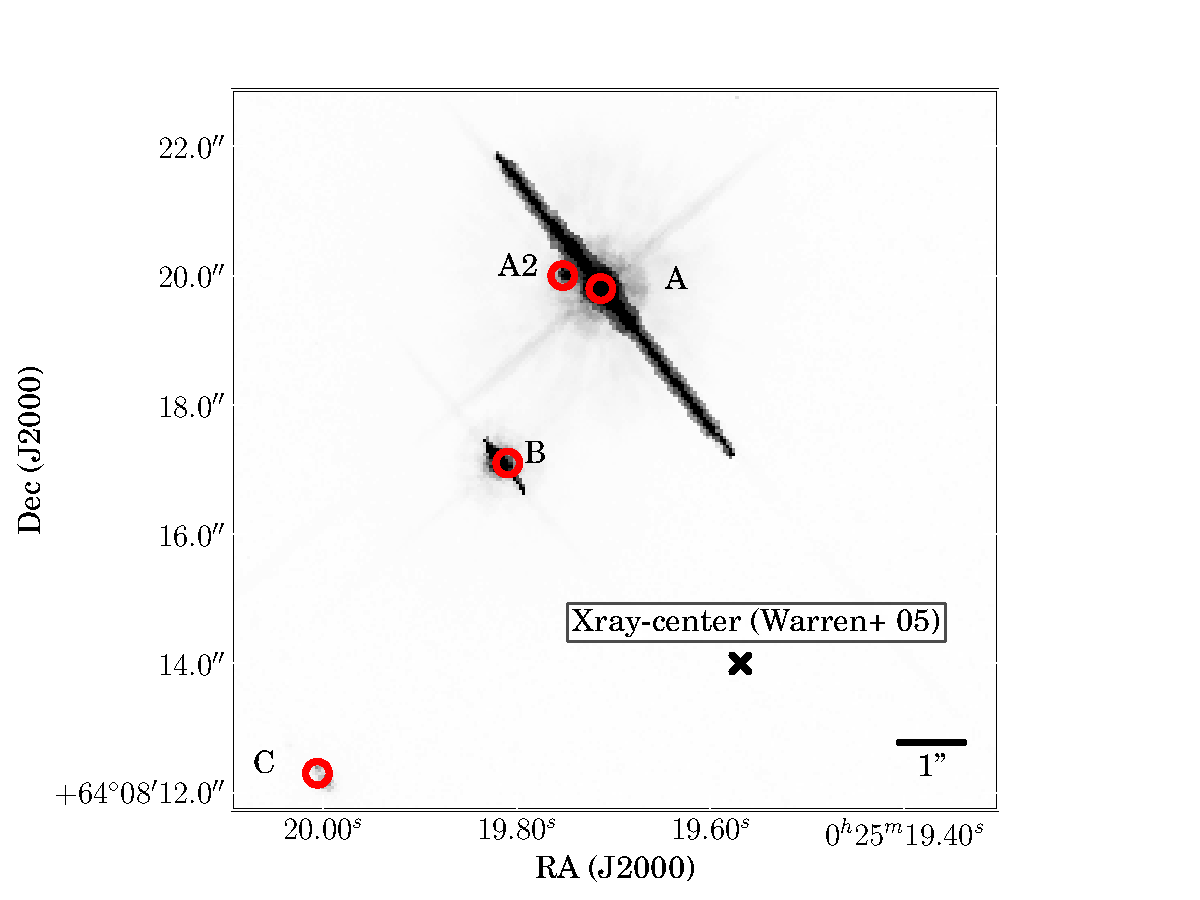
\includegraphics[width=0.7\textwidth]{chapter_conclusion/plots/overview_sn1572_a2.pdf} 
   \caption{Overview of inner region of the remnant of SN1572. All labelled stars except Star-A2 have existing high-resolution spectra. Tycho-A2 is located very close to Tycho-A (0.6\arcsec). Spectroscopy can only be obtained with adaptive optics in the infrared.}
   \label{fig:stara2_overview}
\end{figure}

The bottom line for both SN1572 and SN1006 seems to be: No bright progenitors. There are as always caveats, but we do think that with current theoretical knowledge and current instrumentation it is not worthwhile to scrutinize these remnants further. The only exception is to undertake photometrically deep observations of these remnants and look for a hot white dwarf. 

\section{The curious case of Kepler}

The last of the young remnants and the most distant one \citep[][estimates a distance of $\ge 6$\,\kpc]{2008ApJ...689..231V}.  The morphology of this remnant is not as clean and spherical as for SN1006 and SN1572 (see Figure \ref{fig:sn1604_observations}). For a long time SN1604 (Kepler's supernova) was also believed to be a \snib, but prominent iron emission in \xray spectra \citep{2007ApJ...668L.135R} suggests this event to be a \snia \citep{1995ApJ...444L..81H}. SN1604 also shows an abundance in nitrogen which is unusual for a \snia. \citet{1991ApJ...366..484B} and \citet{2003A&A...407..249S} suggest that the remnant itself posseses a very high systemic velocity of  $\approx 250\,\kms$. A recent study by \citet{2011arXiv1103.5487C} suggests that a \sd-scenario with an AGB star as a donor would explain all the observed peculiarities. They make the prediction that this star should be visible and very bright post-explosion. 

\begin{figure}[htbp] %  figure placement: here, top, bottom, or page
   \centering
   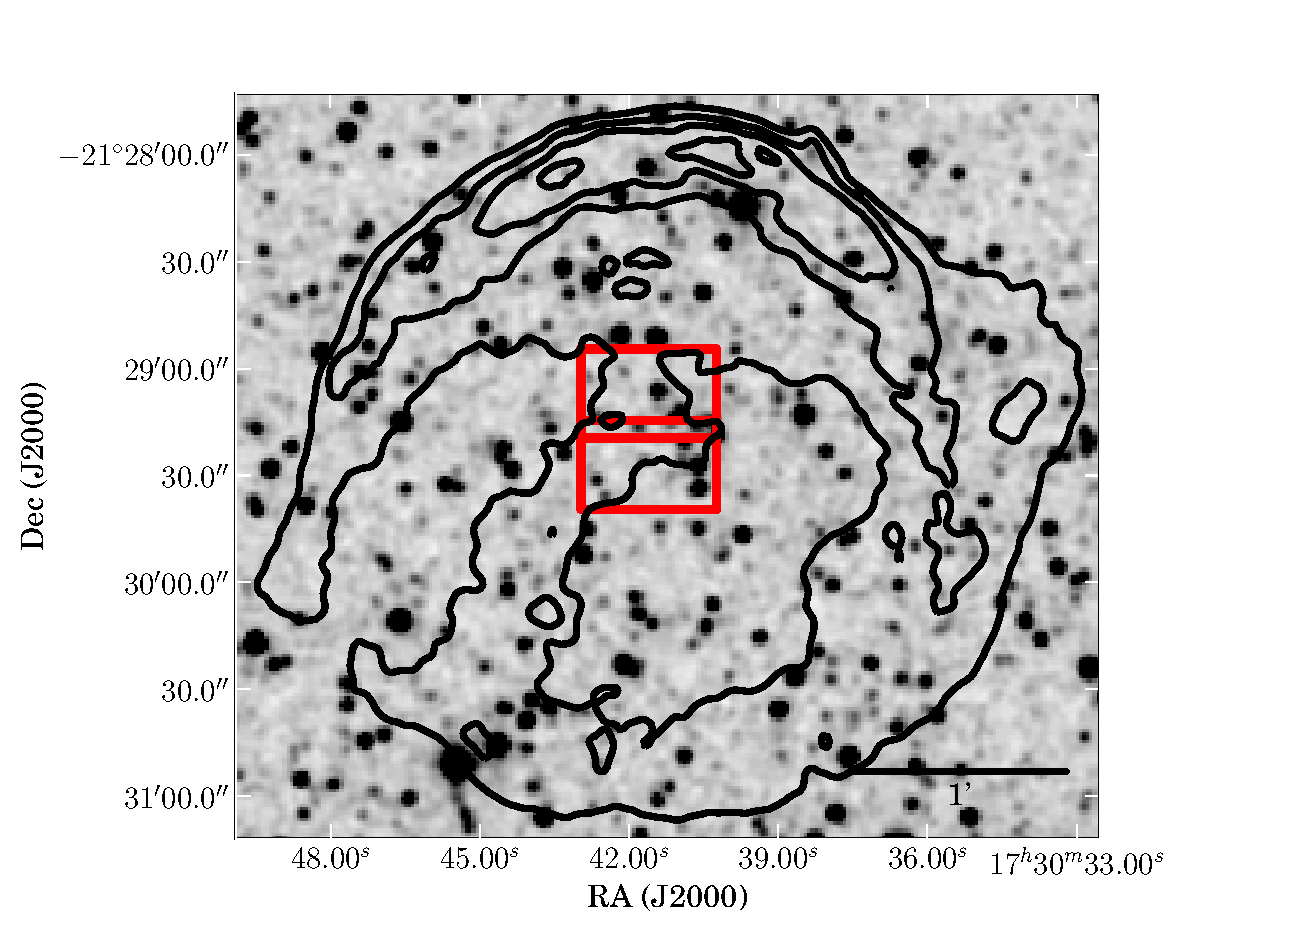
\includegraphics[width=0.7\textwidth]{chapter_conclusion/plots/sn1604_overlay.pdf} 
   \caption{VLA contours of Kepler's remnant (SN1604) overlayed on a \twomass\ image. The red rectangle show the overlapping north and south field of our WiFeS observing campaign.}
   \label{fig:example}
\end{figure}

We have obtained data with the WiFeS integral field spectrograph. The field of view for this instrument. is rectangular with dimensions of $25\arcsec \times 38\arcsec$. We have two overlapping fields that cover all stars at a projected velocity of 1300\,\kms (assuming a distance of 6\,\kpc). Extracting stellar spectra from our poor seeing data ($> 1.5\arcsec$) is technically challenging and we have not invested much time in this project.

\section{Divide et impera}

Maybe finding the progenitors of \sneia\ is too difficult using our current techniques. It might be much easier to employ the successful ``Divide et Impera'' - ``Divide and Conquer'' strategy. By asking many very small questions it might be easier to uncover on the truth than to try to solve this problem at once. We believe that one of these important questions is the mass at which \gls{cowd} explode. There are currently two main scenarios. The favored scenario is the explosion of the \gls{cowd} close to \gls{mchan} (1.38\,\msun). As shown in Chapter \ref{chap:intro} the burning of a 1.38\,\msun \gls{cowd} only produces the right abundance pattern when introducing a delayed detonation. When exploding a 1\,\msun \gls{cowd} this problem does not exist, a detonation of such a star produces the right optical photosheric spectrum. The main problem with these sub-Chandrasekhar mass explosions is that there exists no caveat free theory for the ignition yet. One key to find the explosion mass of any given \snia\ might be the abundance of stable in nebular spectra. In the Chandrasekhar mass case there should be more stable iron, in the case of a sub-Chandrasekhar mass there should be less.

\section{Dalek}

The title of this thesis suggests that \snia-progenitors and their explosions are mutually exclusive fields of research. In the previous section we have however shown that the mass of the white dwarf does have an influence on the yield. This mass is again linked to different progenitor channels. The analysis of spectra might not only help us constrain the elemental yields and explosion energies, but also give us insight into the progenitors. 

In Chapter \ref{chap:dalek} we describe a project to automate the analysis of \snia-spectra. The currently manual operated \gls{mlc}-code is ideal for automating as it strikes the right balance between speed and realism. We researched several numerical optimization strategies for this project before settling on \glspl{ga}. For now we have successfully fitted only one supernova spectrum. We are currently fine-tuning the algorithm and have enlisted the help of experts in the \gls{ga}-field. 

\section{Trouble in Paradise}

During the work of this thesis the field of \snia-research has changed significantly. When we started the donor star search there seemed little doubt in the community about the \sd-scenario. Over the recent years the \sd-channel has been seriously shaken and there has been some newfound support for the \dd-channel. The renaissance of the \dd-scenario, however often comes from the face that the merging of two white dwarfs doesn't provide as strong predictions as the \sd-scenario. This contention has reinvigorated the field of \snia progenitors and makes it a challenging and intriguing area to work in.

New transient and all sky surveys will soon start drowning us in a deluge of data. Currently the astronomical community is ill equipped to deal with such large amounts of data. This is not suprising as most astronomers are experts in physics and not data processing. This problem is not unique to astronomy, more and more fields are gathering much more data than is ever processable by individuals. We believe this is a great opportunity to start cross-disciplinary research. The fundamentals of science (e.g. pattern recognition) are definitley not unique to individual areas. New areas of science like eScience are trying to provide techniques and tools for scientists irregardless of the field. 

We have tried to conduct cross-disciplinary research in automatically fitting \sneia-spectra. Stephan Hachinger (the expert in manual fitting) and me initially have tried using the methods that were tought to us during our undergraduate years in physics (e.g. Newton-Raphson). These methods are still useful for very simple problems, however do not scale to today's highly non-linear problems with many co-dependant variables. Sam Inverso, a computer scientist working many in the area of neuro-science, joined us first and helped us do our first baby-steps in \glspl{ga}. His help has advanced the \gls{dalek} to its present state. In the last half year two new members have joined the team, whose research is in numerical optimization. They are very interested in applying their techniques to ``real world'' problems, which are scarce in the optimization community.

This work definitley tries to show: Multidisciplinary research is not only a buzzword, but can advance individual fields of science much faster than they could advance in isolation.




%% !TEX root =../thesis.tex
\chapter{SN1006}
\label{chap:three}

\lettrine[lines=4]{L}{orem} ipsum dolor sit amet, consectetuer
adipiscing elit. Mauris posuere, elit ac suscipit pulvinar, purus
felis vehicula purus, sed pellentesque arcu nibh eu turpis. Vivamus
volutpat convallis mi. Aliquam varius magna eu urna lacinia
dignissim. Proin venenatis tellus. Fusce pede dui, semper varius,
venenatis vitae, ultrices ac, dolor. Proin diam. Suspendisse eget
purus id leo accumsan scelerisque. Integer rutrum. Etiam risus nibh,
auctor eu, eleifend id, interdum ut, odio. Suspendisse
potenti. Praesent ultricies, mauris convallis vestibulum viverra,
nulla risus porttitor tellus, ut consequat velit nunc at nisi. Nulla
rhoncus nisl quis urna. Morbi sed nunc at tortor rhoncus
iaculis. Lorem ipsum dolor sit amet, consectetuer adipiscing elit. Sed
augue. Nunc molestie.

Maecenas at lectus id nunc bibendum placerat. Suspendisse cursus,
magna vitae blandit bibendum, nisi justo facilisis mi, at faucibus
elit urna id felis. Lorem ipsum dolor sit amet, consectetuer
adipiscing elit. Maecenas risus erat, ornare ac, varius nec, molestie
sed, nulla. Praesent sem urna, sollicitudin in, vulputate at, suscipit
vehicula, lectus. Integer mollis. Curabitur ornare, erat a facilisis
sagittis, risus nulla faucibus diam, at vehicula justo magna nec
urna. Pellentesque rhoncus, turpis eu facilisis molestie, diam ipsum
tristique massa, nec auctor risus diam quis metus. Lorem ipsum dolor
sit amet, consectetuer adipiscing elit. Fusce varius iaculis
neque. Aliquam erat volutpat. Cras sit amet nisi sit amet diam
imperdiet molestie. Quisque nec nisl. Cras nisi velit, pharetra sed,
cursus nec, euismod ac, turpis.

Morbi tincidunt, tellus nec dignissim congue, risus libero
sollicitudin tellus, sit amet porta magna libero sed ante. In id orci
eget nibh ultrices ultrices. Sed feugiat lobortis augue. Integer
nulla. Phasellus lacus diam, ornare id, ornare ut, dictum non,
velit. Ut egestas, risus quis placerat fringilla, nisl nunc tincidunt
ligula, et blandit dui diam vel sem. Morbi mattis turpis et purus
pellentesque accumsan. Mauris enim massa, sollicitudin at, lobortis
quis, ultricies sed, nunc. Pellentesque habitant morbi tristique
senectus et netus et malesuada fames ac turpis egestas. In in
arcu. Vestibulum ante ipsum primis in faucibus orci luctus et ultrices
posuere cubilia Curae; Donec eleifend molestie enim. Etiam justo. Sed
pharetra ultrices lectus. Mauris imperdiet varius purus. Aliquam
commodo adipiscing est. Pellentesque vitae odio fringilla pede viverra
tempor. Vivamus sed sem. Quisque molestie elementum lorem. Proin
aliquam odio vel sapien.

Quisque urna. Praesent scelerisque tortor nec elit. Pellentesque non
urna. Duis non sapien id nunc rutrum facilisis. Donec lectus ipsum,
ullamcorper vel, sollicitudin a, tempor a, sapien. Nam dui. In hac
habitasse platea dictumst. Integer eu ligula id lacus sollicitudin
sodales. Nam aliquam nibh vitae urna gravida rutrum. Aliquam erat
volutpat. Integer gravida mattis tellus. Etiam ipsum lacus, dapibus
id, volutpat eget, vestibulum vel, pede. In odio quam, viverra id,
adipiscing nec, consequat ut, orci. Nunc sit amet neque eu risus
dictum ultrices. Proin sem quam, ullamcorper ut, posuere at, tempus
eget, nibh. Cras ipsum. Phasellus bibendum purus eu enim. In hac
habitasse platea dictumst. Praesent eget leo ac sem congue sodales.

Nunc malesuada turpis vitae neque. Donec sollicitudin libero vel
nisi. Aliquam congue sem sed est. Integer eget ipsum. Nam eu
mauris. Aliquam vehicula tempor nulla. Duis faucibus ornare
elit. Vivamus nunc. Phasellus placerat, orci non blandit scelerisque,
neque urna faucibus justo, non gravida pede sem a urna. Sed eget arcu
eget enim pellentesque tincidunt. Cum sociis natoque penatibus et
magnis dis parturient montes, nascetur ridiculus mus. In in nulla sed
est venenatis sagittis. Mauris nibh orci, adipiscing in, blandit quis,
vulputate vitae, tortor. Quisque venenatis. Ut leo quam, pellentesque
vitae, dictum ut, vestibulum at, turpis. Aliquam id urna. Vestibulum
nunc mauris, facilisis sed, molestie quis, consequat non, dui.

Duis id metus et tortor viverra varius. Vivamus consequat. Sed
bibendum ultricies lectus. Pellentesque vulputate orci vitae
augue. Vivamus dignissim pharetra mauris. Lorem ipsum dolor sit amet,
consectetuer adipiscing elit. Vestibulum purus purus, commodo in,
consequat eu, lobortis eu, sem. Proin volutpat, pede eu imperdiet
bibendum, nulla odio lobortis eros, eu aliquet neque nunc eu
enim. Donec non nunc. Aliquam erat volutpat. Ut cursus fermentum orci.

Class aptent taciti sociosqu ad litora torquent per conubia nostra,
per inceptos himenaeos. Donec ante eros, porttitor vel, pellentesque
sit amet, laoreet ut, velit. Vestibulum sit amet turpis sed lorem
vestibulum vulputate. Maecenas sed orci in ante pharetra accumsan. Sed
id nibh. Pellentesque dapibus varius neque. Pellentesque habitant
morbi tristique senectus et netus et malesuada fames ac turpis
egestas. Nullam ultrices augue. Lorem ipsum dolor sit amet,
consectetuer adipiscing elit. Etiam convallis placerat
tortor. Suspendisse potenti. Mauris porttitor, justo et mollis
dapibus, dui nunc accumsan dolor, quis sollicitudin est nisi at
libero. Donec sollicitudin eros sed neque. Nunc at quam.

Donec id arcu. Sed vel sapien sit amet metus vestibulum
fringilla. Etiam fringilla ligula at arcu. Donec bibendum sem et
quam. Nam diam mauris, malesuada vel, placerat a, fermentum sit amet,
lectus. Cras venenatis justo nec leo. Aliquam vulputate erat. Cras
turpis. Cras gravida. Aliquam erat volutpat. Sed porta pretium
ligula. Mauris viverra, nisi euismod vulputate lobortis, est tortor
consectetuer arcu, at congue quam ipsum sit amet sem. Cum sociis
natoque penatibus et magnis dis parturient montes, nascetur ridiculus
mus. Mauris eget dolor.

Suspendisse pulvinar. Suspendisse felis nisl, mattis sed, facilisis
at, laoreet vitae, magna. Suspendisse potenti. Pellentesque et ligula
vel mauris suscipit vestibulum. Phasellus eros sem, volutpat at,
feugiat ut, aliquam sed, augue. In hac habitasse platea
dictumst. Suspendisse suscipit. Cum sociis natoque penatibus et magnis
dis parturient montes, nascetur ridiculus mus. In lectus dolor,
commodo non, ultricies eu, scelerisque at, orci. Nulla
semper. Suspendisse potenti. Donec orci diam, pellentesque tristique,
tempus eget, tincidunt in, dolor. Maecenas tristique vehicula
risus. Integer vitae nisi. Aenean sed enim eu nisl suscipit
scelerisque. Integer non metus. Donec dui erat, bibendum eu, suscipit
eu, facilisis non, erat. Morbi dapibus pede id justo. Fusce lobortis
volutpat enim.

Morbi leo turpis, facilisis in, ultrices vel, adipiscing ut,
erat. Praesent ligula. Maecenas quis velit in orci adipiscing
aliquam. Quisque at pede. Integer at odio. Pellentesque feugiat tellus
sed risus. Mauris et turpis. Nam sodales. Suspendisse mollis tincidunt
sapien. In ac sapien et purus sollicitudin ultricies. Integer eget
sapien quis ligula commodo egestas. Nulla aliquam, odio sed tincidunt
blandit, pede dolor gravida nunc, nec condimentum lorem nulla eget
dui.  




%
\bibliographystyle{astroads}
\bibliography{thesis}

\end{document}
